\documentclass[11pt]{article}
\usepackage[a4paper, top=4cm, bottom=3cm, left=3cm, right=3cm]{geometry}
\usepackage{geometry} % see geometry.pdf on how to lay out the page. There's lots.
\geometry{a4paper} % or letter or a5paper or ... etc
% \geometry{landscape} % rotated page geometry
\usepackage[english]{babel}
%\usepackage[utf8]{inputenc}
%\usepackage{accents}
\usepackage{graphicx}
\usepackage{array}
\usepackage{multirow}
%\usepackage{mathptmx}
%\usepackage{amsmath}
%\usepackage{makeidx}
\usepackage{verbatim}
\usepackage{amssymb}
\usepackage{latexsym}
\usepackage{comment}
\usepackage{sectsty}
\usepackage{accents}
\usepackage{natbib}
\usepackage{caption}
% See the ``Article customise'' template for come common customisations
\newcolumntype{x}[1]{{\centering\hspace{0pt}}p{#1}}

% By Simon ==================================================


\newcommand{\simon}[1]{\vspace{1em}(\emph{Simon: #1})\vspace{1em}}

%TIKZ====
\usepackage{tikz}
\usetikzlibrary{arrows,shadows,petri,positioning}
%\usetikzlibrary{fit}					% fitting shapes to coordinates

% End by Simon =============================================


\title{ICT for Basic Service Delivery - Case Study: Water Sector in Uganda}
\author{
\small{Ikae Catherine Omal}\\
\small{School of Computing and Informatics Technology, University of Makerere, Uganda}\\ \small{\textit{ikae.catherine@cit.mak.ac.ug}}\\
}

\date{\today}

\begin{document}
\maketitle

\begin{abstract}
To be completed
\end{abstract}



%%%%%%%%%%%%%%%%%%%%%%%%%%%%%%%%%%%
%Introduction
\section{Background, research hypotheses and objectives}\label{background}
Should include defined and justified objective (point2), problem definition (point3) and a short introduction of project description (point4) and the institutional framework and partnership (point9)

\simon{I added two temporary list just for myself}

\paragraph{Temporary: Bigger Picture}
\begin{enumerate}
 \item Provide better water service through mobile ICT in rural Uganda
 \item Collect data (context, location, text) from mobile users in rural Uganda
\end{enumerate}


\paragraph{Temporary: Objectives}
\begin{itemize}
\item[(i)] an analysis of the current situation (who are the people using phones, current phone penetration and usages, barriers to usage, type of phones used, frequency of ICT communication, forms of communication related to water issues…)
\item[(ii)] the design of the communication channels to provide the bottom-up information on water: nature of the message (sms, mail, voice…), the language used, the actions required (forms, dialed-in choice selection, special number-to-action, voice messengers…)
\item[(iii)] the design of the response with the same problems and criteria as for (ii)
\item[(iv)] the ability to test for the information effectiveness and efficiency of the different response/feedback solutions proposed
\item[(v)] the ability to test for some social incentives, through peer pressure or some forms of "gamification"
\end{itemize}


\section{State of research in the field}\label{state_of_research}
Should cover state of research and references (point3), and innovativeness of research/ research methodology (point4) + corresponding logical framework (whatever that is)

\simon{To Do}

\begin{itemize}
 \item jana formerly txteagle
 \item FrontlineSMS
 \item RapidSMS
 \item ushahidi
 \item h20initiative
 \item rwsn.ch
 \item m4water.org
 \item waterpointmapper.org
\end{itemize}


\section{Methodology}\label{methodology}
\subsection{Methodology}\label{metho}
Should give in full details the methodology to be used (point4)

\begin{figure}
\begin{center}
 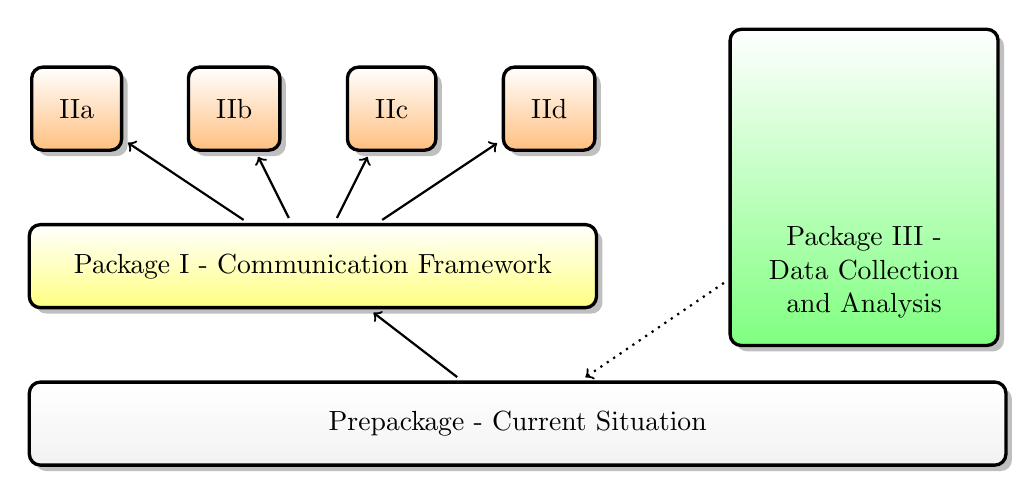
\begin{tikzpicture}[node distance=1.5cm, shorten >=2pt, shorten <=2pt, thick, auto]


\tikzstyle{box} = [
    rectangle,rounded corners,draw=black, top color=white, very thick, inner sep=1em, minimum size=3em,drop shadow]

 
\node[box, bottom color=gray!10, text width = 11.7cm, text centered] at (-1.4,0) (prepackage) {Prepackage - Current Situation};

\node[box, bottom color=yellow!50, text width = 6.5cm, text centered] at (-4,2) (packagei) {Package I - Communication Framework};

\node[box, bottom color=green!50,  text width = 2.7cm, text height = 2.4cm, text centered] at (3,3) (packageiii) {Package III - Data Collection and Analysis};


\node[box,  bottom color=orange!50] at (-7,4) (packageiia) {IIa};

\node[box,  bottom color=orange!50] at (-5,4) (packageiib) {IIb};

\node[box,  bottom color=orange!50] at (-3,4) (packageiic) {IIc};

\node[box,  bottom color=orange!50] at (-1,4) (packageiid) {IId};



\path[->]
  (prepackage) edge (packagei)
  (packagei) edge (packageiia)
  (packagei) edge (packageiib)
  (packagei) edge (packageiic)
  (packagei) edge (packageiid)
;

\path[->, dotted]
  (packageiii) edge (prepackage)
;


\end{tikzpicture} 
\end{center}
\caption{Research packages hirarchy}
\label{tikz:researchpackages}
\end{figure} 

Champanis and Rivett \cite{champanis2012reporting} state: \begin{quote}
``Based on our experience and focus on rural environments, our
approach to ICT development has been that the investigation of
the local context and solutions responding to local needs are more
valuable and sustainable than a general “one-size-fits-all” design.
Whilst this speaks against the notions of “scalability”, which is
usually a desired outcome for IT solutions, we believe that rural
and under-resourced environments require a more detailed and
customised solution.''\end{quote} 

A set of research packages is presented that allows to build up a well tailored but still scalable solution that - beside of helping people directly -  gives space to investigate on research relevant questions in the field of computer science and further sociology, development aid and economics. 

Figure~\ref{tikz:researchpackages} explains the research packages hierarchy: The small Prepackage analyses the context. In Package I the main framework for future project plug-ins is designed. The actual scientific part from a computer science perspective is done in Package II whose subpackages can be implemented individually. Package III is a parallel ongoing process that profits from improvements in Packages I\&II.


\subsubsection*{Prepackage: Analysis of the current situation}
\paragraph{Goal} Get an overview of mobile ICT usage and water management in rural Uganda
\paragraph{Method}
In the field of mobile ICT information is aggregate from cooperation with governmental institutions, local service provides and by detailed literature study:
\begin{enumerate}
 \item Distribution of cell phones (by model, user age, area)
 \item Usage distribution (by time, frequency and service)
 \item Analysis of finances (income per user, cost of different services per user, money spent for different services per user)
 \item Analysis of technology (cellular network standards, cell sizes, user per cells, quality of service, future investments, availability of electricity)
 \item Analysis of hindrances for a more frequent usage (finances, easy of use, illiteracy, privacy concerns)
\end{enumerate}
In the field of drinking water additional input comes from partnership with local NGOs.
\begin{enumerate}
 \item Analysis of the drinking water need amongst population and its challenges
 \item Further data will be collected during the project as a result of Package III
\end{enumerate}







\subsubsection*{Package I: Design of a communication channel}
\paragraph{Goal} Design a inter-user communication channel that is user friendly, low-cost, reliable, secure and information rich
\paragraph{Method} A first substep evaluates different communication channels. Text-, graphical- and voice based methods are compared on different generations of phones. Depending on their connection standards (GSM, GPRS, 3G) and application platforms supported (SMS, Java Me, Android) best possible options are chosen. Challenges occur in the following areas:
\begin{itemize}
 \item Low cost feature phones (``a modern low-end mobile phone that is not a smart phone'' [Wikipedia]) are widely available in Uganda. Their drawback is that software has to be implemented manufacturer depending and in general allows just limited functionality \cite{champanis2012reporting}.
 \item Access to provider data (calls with user id, text messages, cell info) is difficult to obtain. A possible solution is to use just mobile data services and transfer messages based on an extra developed service.
 \item Literacy rate of Uganda is around 66 percent [Wikipedia]. Tailored solutions for illiterates have successfully been implemented \cite{brown2012water}. By developing special input methods, one has to be aware that a very important reason for people to buy a phone is due to its associated status and not its features \cite{knoche2012text}.
 \item Low cost transmission is necessary to achieve a high user participation. Prices for SMS make up a higher percentage of the monthly budget than in high income countries. An alternative approach is to provide hardware and airtime to selected user group in order to conduct studies.
 \item Free hardware and airtime is likely to be misused. Champanis and Rivet report that ``Users would fill up the phone with music and video downloads'' \cite{champanis2012reporting} to an extend that it is not usable for the experiment anymore.
 \item User trust and information security is one of Africas biggest challeng, this due to weak privacy laws, user awareness, political instability and not maintained software \cite{goodman2010coming}.
\end{itemize}

In a second substep we analyse the information flow needed to provide a water quality information and monitoring network. The implementation (third substep) completes Package I. To the moment it remains an open question if a self designed device for data transmission over the mobile network would fulfil this purpose even better than a cell phone based service. 

The success of such an system is unpredictable. Hence we suggest an iterative approach based on trial and error method. Lessons learned from other projects are considered and results reported to the community.



\subsubsection*{Package IIa: Quality control}
\paragraph{Goal} Achieve high quality information collected at a centralised agent but also sent to individual receivers 
\paragraph{Method} According to \cite{birnbaum2012automated} supervised and unsupervised machine learning methods are feasible to classify manually generated data in health surveys in Tanzania and Uganda. Widely used machine learning algorithms could be modified in order to not just classify but rather rate user message according to a scale of trust. Additionally the knowledge of the crowd is used to label messages and hence a  supervised learning on initially unlabelled data is performed - similar to a supervised spam filter. Out of this, a general trust giving and learning (human and machine based) distributed network could be generated.

This contains the following areas of risk:

\begin{itemize}
 \item The reported lack of data quality in surveys in low income countries could also be the result of the normally used top-down approach \cite{birnbaum2012automated}, whereas a bottom-up approach  (where users have a personal interest on the quality of the data) might not even, or at least less face this problem.
 \item The question resides if a machine learning solution for such a difficult task is an actual benefit for a country where human workforce is cheap (and jobs needed) and technology expensive. We would not be surprised if a mixed solution - highlighting suspicious messages machine- and final classification human based - might be the best solution.
\end{itemize}







\subsubsection*{Package IIb: Context analysis}
\paragraph{Goal} Gather context data of users and messages and provide information accordingly

\paragraph{Method}
Four different fields of study can be divided:
\begin{description}
 \item [User context] Albeit low cost feature phones provide just limited sensor functionality, they allow nevertheless access to basic context information like position (Cell site or GPS), time and number of contacts (address book). Out of this, additional contextual information like weather condition can be added.
 \item [Message content and context] To get a meaningful information transfer on water quality between humans and a machine it is mandatory to understand the content of a message either by the use specific questioning and answer mechanisms (e.g. input form) or by mining data out of unspecific messages. Later is current field of research, e.g in the area of text messages \cite{aggarwal2012mining}. This gives a high degree of freedom to test, redesign and evaluate state of the art algorithms. Once functioning methods are available, they can be used as well to support subfield one (User context) by mining additionally user context information out of the exchanged messages. 
 \item [Context information provision] Having filtered data, most relevant information is provided to the users, (e.g. closest working water source, closest available mechanic, water shortage in specific area, water preparation information). The task is either done by a machine- or human agent for which a specific interface would be designed.
 \item [Contextual information presentation] The gained context information can be used to present the information in more readable way, e.g. by using specific graphics.
\end{description}

Risks in this package are low since goals and functionality are scalable depending on success of basic experiences.


\subsubsection*{Package IIc: Water mapping}
\paragraph{Goal} Map water status information on the web
\paragraph{Method} Together with local partners\footnote{http://wwww.spactialcollective.com} an interface is designed that allows spacial mapping on a web platform.

\subsubsection*{Package IId: Incentives and gamification}
\paragraph{Goal} Analyse methods to get more user participation
\paragraph{Method}
The so far described intelligent network is improved by testing and comparing different incentives and gaming approaches. Knowledge from Package IIb is used to create social incentives. Comparative studies similar to \cite{blaschkeextrinsic} are performed. 

\simon{@Jonathan: Maybe you can add here something, this is definitely not (yet) my field of expertise}

\subsubsection*{Package III: Data collection and analysis}
\paragraph{Goal} Use the built system to collect data and use it for further improvements
\paragraph{Method}

\begin{itemize}
 \item If successful, the platform from Project I and the modules from Project II provide a large amount of data that can be used even outside the scope of the water sector and computer science. Since data is accumulated from the first implementation of Project I, this is a parallel ongoing process.
 \item The interface to a centralised human agent (introduced Package IIb) can be used to conduct surveys where the data accumulated from the bottom-up network does not provide the necessary information.
 
 \item Information collected on water access (average distance travelled for water access, pump durability, water well users profile) can be used to improve Package I\&II.
\end{itemize}



\subsection{Chances and risk associated with selected methodology}\label{risk}
Critical assessment of chances and risks (points8)

\simon{Is actually included already in Section~\ref{metho}, i.e. merge Section~\ref{metho} and \ref{risk}}

\section{Organization}\label{organization}
Should describe in details the institutional framework and the partnership, explaining the contribution of all involved partners (point 5). Clear presentation of the supervision and backstopping (point 6).
\section{Expected results}\label{expected}
Expected results and strategy for their implementation (method or product to be developed and its relevance to end users) (point9)
\section{Budget}
Detailed budget for each year of the scholarship, differentiating all funding sources including those of the ETH chair and partner contributions (financial or in-kind) (point10)


\bibliographystyle{plain}
\bibliography{proposal07022013_jg}


\end{document}